%%=============================================================================
%% Netwerkconcepten
%%=============================================================================

\chapter{\IfLanguageName{dutch}{Computernetwerk concepten}{Computer network concepts}}%
\label{ch:computernetwerk-concepten}

\section{Inleiding}
\label{netwerk_inleiding}

Tegenwoordig heeft vrijwel elke server toegang nodig tot het netwerk om te kunnen communiceren met andere servers of clients.
Dit vormt een essentieel onderdeel van de serverfunctionaliteit, aangezien het zonder netwerkconnectiviteit niet bereikbaar zou zijn.
Om deze connectiviteit te realiseren, zijn er verschillende concepten en technologie\"en beschikbaar die kunnen worden toegepast.

In dit hoofdstuk zullen we enkele van deze concepten en technologie\"en bespreken die ons later zullen helpen bij het identificeren van wat het beste kan worden opgenomen in ons configuratie-inventaris.

\section{Netwerkinterface}
\label{netwerk_netwerkinterface}

Een netwerkinterfacecontroller (NIC) is een hardwarecomponent die een computer in staat stelt te communiceren met andere computers via een netwerk.
Het bereidt de gegevens voor die moeten worden verzonden en ontvangen, en zet deze om naar een formaat dat via het netwerk kan worden verzonden.
Een systeem kan meerdere NIC's bevatten; bijvoorbeeld een laptop kan zowel een draadloze NIC voor WiFi als een bedrade NIC voor Ethernet hebben~\autocite{hypponen2021securing}.
Binnen het OSI-model maakt de NIC deel uit van de fysieke laag.

Voordat een NIC kan worden gebruikt, moet de juiste netwerkdriver zijn geïnstalleerd op het systeem.
Deze driver stuurt de onderliggende hardware aan en zorgt ervoor dat deze correct communiceert met het besturingssysteem.
Daarnaast is de driver verantwoordelijk voor het toewijzen van adressen, het aanpassen van transmissieparameters en het waarborgen van het netwerkverkeer~\autocite{hypponen2021securing}.

\section{Netwerkprotocollen}
\label{netwerk_netwerkprotocollen}

Netwerken zijn bijna altijd hi\"erarchisch opgebouwd en bestaan uit verschillende lagen.
Elke laag heeft zijn eigen specifieke functie en is verantwoordelijk voor een bepaald aspect van de communicatie.
Het OSI-model (Open Systems Interconnection model) is een referentiemodel dat deze lagen beschrijft en de communicatie tussen systemen mogelijk maken.
Dit model heeft de volgende lagen~\autocite{tanenbaum1981network}:

\begin{enumerate}
    \item Fysieke laag
    \item Data link laag
    \item Netwerklaag
    \item Transportlaag
    \item Sessielaag
    \item Presentatielaag
    \item Applicatielaag
\end{enumerate}

Dit deel zullen enkele van de belangrijkste protocollen en technologie\"en worden besproken die worden gebruikt in computernetwerken.

\subsection{Internet Protocol versie 4}
\label{netwerk_ipv4}

IPv4, voluit het Internet Protocol versie 4 genoemd, is de vierde iteratie van het Internet Protocol en wordt ingezet op de netwerklaag van het OSI-model, als onderdeel van de TCP/IP-protocolstack.
Dit protocol, ontworpen door DARPA (Defense Advanced Research Projects Agency), is momenteel het meest gangbare Internet Protocol.
Het vormt de ruggengraat van het internet en faciliteert de verzending van pakketten van de ene computer naar de andere, via een reeks van onderling verbonden netwerken.

In de werking van het protocol worden gegevens van de bovenliggende lagen ge\"encapsuleerd in pakketten, die vervolgens over het netwerk worden verzonden.
Samen met de IPv4-header, die metadata bevat over het pakket, worden de gegevens doorgegeven van netwerk naar netwerk, totdat ze hun bestemming bereiken of de maximale levensduur bereiken (aangeduid als TTL, oftewel Time to Live, zoals te zien in figuur~\ref{fig:network-ipv4-header}).
Wanneer de TTL is verstreken, wordt het pakket verwijderd en wordt er een ICMP-pakket teruggestuurd naar de afzender om dit aan te geven~\autocite{dordal2020}.

\begin{figure}[h!]
    \begin{center}
        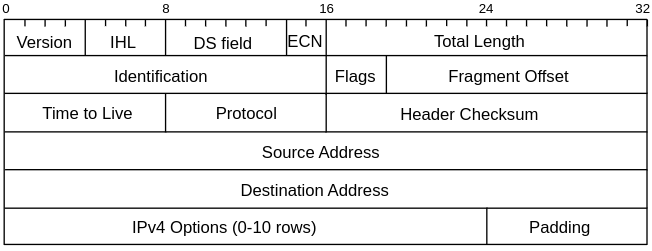
\includegraphics[width=300pt]
        {./graphics/network/ipv4-header.png}
        \caption{\label{fig:network-ipv4-header}Diagram van een IPv4 header~\autocite{dordal2020}.}
    \end{center}
\end{figure}

Ipv4 maakt gebruik van 32-bit adressen en ondersteunt ongeveer \(2^{32}\) adressen, wat neerkomt op ongeveer 4,3 miljard unieke adressen.
Een adres wordt gelinkt aan een specifieke netwerkinterface en maakt het mogelijk om deze interface te identificeren en te lokaliseren binnen een netwerk.
Wanneer we spreken over een IPv4-adres, verwijzen we meestal naar een van de volgende notaties:

\begin{itemize}
    \item \texttt{192.168.0.82}
    \item \texttt{127.0.0.1}
\end{itemize}

Dit zijn zogenaamde dotted-decimal notaties, waarbij elk octet van het adres wordt gescheiden door een punt.
Als we echter een adres in een binair formaat willen weergeven, kunnen we dit doen door elk octet te converteren naar een 8-bit binair getal en deze aan elkaar te koppelen.
Dit resulteert in volgende notatie, respectievelijk voor de bovenstaande voorbeelden:

\begin{itemize}
    \item \texttt{11000000.10101000.00000000.01010010}
    \item \texttt{01111111.00000000.00000000.00000001}
\end{itemize}

Deze IP-adressen kunnen we verdelen in twee delen: het netwerkdeel en het hostdeel.
Neem bijvoorbeeld het adres \texttt{192.168.0.82}, dat we kunnen opsplitsen in \texttt{192.168.0} en \texttt{82}.
Deze scheiding is nuttig om vast te stellen welke hosts zich in hetzelfde netwerk bevinden en welke niet.
De splitsing wordt bepaald door een subnetmask, dat aangeeft welke bits van het adres het netwerkdeel vormen en welke het hostdeel.
In het geval van \texttt{192.168.0.82} zou het subnetmask bijvoorbeeld \texttt{255.255.255.0} zijn, wat overeenkomt met 24 bits voor het netwerkdeel en 8 bits voor het hostdeel.
Een andere notatie die wordt gebruikt, is de CIDR-notatie, waarbij het aantal bits dat het netwerkdeel vormt direct wordt aangegeven.
Voor het bovenstaande voorbeeld zou dit \texttt{192.168.0.82/24} zijn.

\subsection{Internet Protocol versie 6}
\label{netwerk_ipv6}

IPv6, oftewel Internet Protocol versie 6, vertegenwoordigt de opvolging van IPv4 en is ontworpen om de beperkingen van zijn voorganger aan te pakken.
Met de exponenti\"ele groei van het internet en de groeiende vraag naar meer adressen werd duidelijk dat het beschikbare aantal IPv4-adressen ontoereikend zou zijn.
Als reactie hierop werd IPv6 ontwikkeld, dat gebruikmaakt van 128-bit adressen en naar schatting ongeveer \(2^{128}\) unieke adressen ondersteunt.

Dit protocol functioneert op de netwerklaag van het OSI-model en vertoont overeenkomsten met IPv4 in termen van werking.
Het onderscheidt zich echter door zijn adressering, die in een andere notatie wordt weergegeven en meer bits bevat.
Bovendien bestaat de header van een IPv6-pakket uit 40 bytes, wat tweemaal zo groot is als de 20 bytes van een IPv4-header, zoals geïllustreerd in figuur~\ref{fig:network-ipv6-header}~\autocite{dordal2020}.

\begin{figure}[h!]
    \begin{center}
        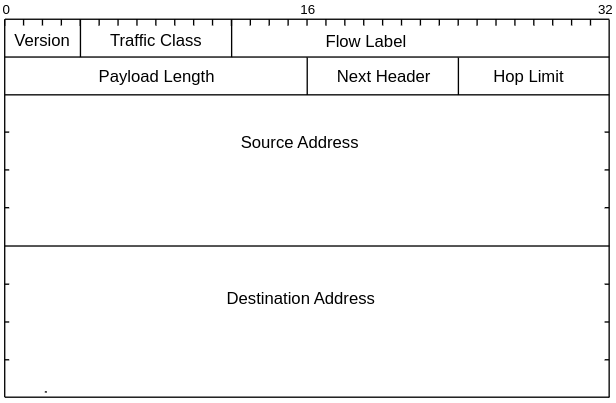
\includegraphics[width=300pt]
        {./graphics/network/ipv6-header.png}
        \caption{\label{fig:network-ipv6-header}Diagram van een IPv6 header~\autocite{dordal2020}.}
    \end{center}
\end{figure}

De IPv6-header verschilt van zijn IPv4-tegenhanger. Zo ontbreekt bijvoorbeeld het TTL-veld en wordt dit vervangen door een veld genaamd Hop Limit.

IPv6 maakt gebruik van adressen die 128 bits lang zijn en worden weergegeven in een hexadecimale notatie, zoals in het volgende voorbeeld:

\begin{itemize}
    \item \texttt{fe80::7255:7ef:9d20:a8ae}
    \item \texttt{::1} (IPv6 equivalent van \texttt{127.0.0.1})
\end{itemize}

\subsection{Routingtabellen}
\label{netwerk_routeringstabel}

Het doorsturen van pakketten van de ene host naar de andere gebeurt via routers, die fungeren als tussenstations in het netwerk.
Deze routers houden elk hun eigen routingtabel bij, ook wel bekend als een IP-forwardingtabel~\autocite{dordal2020}.
Computers houden zelf ook een routingtabel bij om te bepalen naar welke router ze pakketten moeten sturen om hun bestemming op een zo efficiënt mogelijke manier te bereiken, zoals te zien is in listing~\ref{lst:linux-routering}.

\begin{listing}
  \begin{minted}[linenos,tabsize=4,breaklines]{console}
[anton@fedorable ~]$ ip route
default via 192.168.0.1 dev wlo1 proto dhcp src 192.168.0.82 metric 600
192.168.0.0/24 dev wlo1 proto kernel scope link src 192.168.0.82 metric 600
  \end{minted}
  \caption{Uitvoer van het commando \texttt{ip route} op een Linux-systeem, dat de routeringstabel toont.}
  \label{lst:linux-routering}
\end{listing}

Zoals te zien is in listing~\ref{lst:linux-routering}, bevat de routingtabel routes naar specifieke netwerken, die elk een doeladres en een netwerkinterface bevatten.
Op basis hiervan wordt een pakket doorgestuurd naar de juiste router, die het vervolgens verder doorstuurt naar de volgende router of naar de bestemming.
IP-forwardingtabellen bevatten netwerkvoorvoegsels als bestemmingen, zoals beschreven in de tekst.
Het matchen van een pakketadres met een vermelding in de forwardingtabel vereist vergelijking van de voorvoegsels, niet alleen eenvoudige gelijkheidscontrole.

\subsection{User Datagram Protocol}
\label{netwerk_udp}

UDP, voluit User Datagram Protocol, is een ander protocol dat, net als TCP, opereert op de transportlaag van het OSI-model.
Het onderscheidt zich doordat het een eenvoudig protocol is dat communicatie mogelijk maakt tussen twee hosts zonder dat er eerst een verbinding hoeft te worden opgezet.
Dit betekent dat het een connectionless protocol is, in tegenstelling tot TCP, waarover we later zullen praten.

Het staat bekend als een lichtgewicht protocol dat snel en effici\"ent werkt, maar geen garanties biedt voor de levering van pakketten.
Wanneer een zender een pakket naar de ontvanger stuurt, is er geen bevestiging van ontvangst, wat betekent dat pakketten verloren kunnen gaan zonder dat de zender hiervan op de hoogte is.

UDP communiceert op basis van datagrammen, die onafhankelijk van elkaar worden verzonden en ontvangen.
Binnen elk datagram is er een header van 8 bytes aanwezig, die is onderverdeeld in vier gelijke velden van elk 16 bits.
De eerste 16 bits vertegenwoordigen de bronpoort, die waarden kan hebben tussen 0 en 65535 en applicaties identificeert.
Het tweede deel van de header bevat de doelpoort, die eveneens varieert van 0 tot 65535 en de bestemmingsapplicatie identificeert.
Vervolgens is er een veld van 16 bits voor de lengte van het datagram en een checksum van 16 bits om de integriteit van het pakket te waarborgen~\autocite{dordal2020}.
Een voorbeeld van een UDP-header is te zien in figuur~\ref{fig:netwerk-udp-header}.

\begin{figure}[h!]
    \begin{center}
        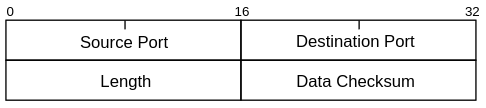
\includegraphics[width=200pt]
        {./graphics/network/udp-header.png}
        \caption{\label{fig:netwerk-udp-header}Diagram van een UDP header~\autocite{dordal2020}.}
    \end{center}
\end{figure}

\subsection{Transmission Control Protocol}
\label{netwerk_tcp}

Net als UDP is TCP, staande voor Transmission Control Protocol, een essentieel protocol voor communicatie tussen hosts op een netwerk.
Toch verschillen de twee protocollen in hoe ze gegevens verzenden en ontvangen.
In tegenstelling tot UDP is TCP een connection-oriented protocol, wat betekent dat het eerst een verbinding opzet voordat gegevens worden uitgewisseld.
Dit gebeurt via de zogenaamde three-way handshake, waarbij beide partijen communiceren om ervoor te zorgen dat gegevens correct en in de juiste volgorde worden afgeleverd.

Om communicatie via TCP mogelijk te maken, stuurt een van de hosts een SYN-pakket naar de andere host.
Wanneer de ontvangende host dit pakket ontvangt, stuurt deze een SYN-ACK-pakket terug naar de zender.
Vervolgens stuurt de zender een ACK-pakket terug, waarna de verbinding tot stand is gebracht en gegevens kunnen worden uitgewisseld~\autocite{hypponen2021securing}.
Dit proces wordt geïllustreerd in figuur~\ref{fig:netwerk-tcp-handshake}.

\begin{figure}[h!]
    \begin{center}
        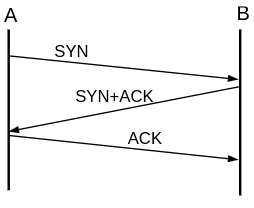
\includegraphics[width=100pt]
        {./graphics/network/tcp-handshake.png}
        \caption{\label{fig:netwerk-tcp-handshake}TCP three-way handshake~\autocite{dordal2020}.}
    \end{center}
\end{figure}

De TCP-header is ook complexer dan die van UDP, met een totale lengte van 20 bytes, zoals weergegeven in figuur~\ref{fig:netwerk-tcp-header}.
Net als bij UDP beginnen de bron- en doelpoorten de header, die vari\"eren van 0 tot 65535.
Daarna volgt een veld voor de sequentienummering, dat de volgorde van de gegevens bepaalt.
Verder is er een veld voor de bevestigingsnummering, dat wordt gebruikt om te bevestigen dat gegevens correct zijn ontvangen.
Ook bevat de header weer een checksum om de integriteit van het pakket te waarborgen~\autocite{dordal2020}.

\begin{figure}[h!]
    \begin{center}
        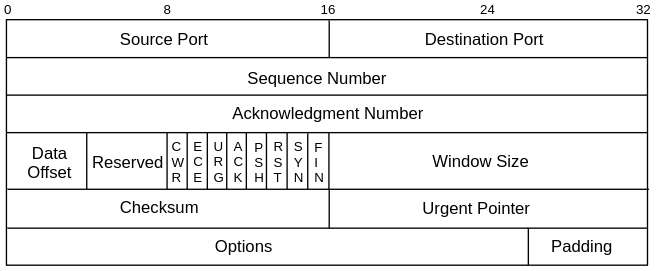
\includegraphics[width=300pt]
        {./graphics/network/tcp-header.png}
        \caption{\label{fig:netwerk-tcp-header}Diagram van een TCP header~\autocite{dordal2020}.}
    \end{center}
\end{figure}

\subsection{Domain Name System}
\label{netwerk_dns}

Eerder werd al benadrukt dat elke host op een netwerk minstens één IP-adres heeft.
Hoewel deze IP-adressen essentieel zijn voor communicatie op internet, zijn ze niet bijzonder gebruiksvriendelijk.
Het onthouden en gebruiken van lange reeksen cijfers is niet praktisch in het dagelijks gebruik.
Om deze uitdaging aan te pakken en het internet toegankelijker te maken, is het Domain Name System (DNS) ontwikkeld.

Het hele protocol zou men kunnen vergelijken met een telefoonboek, waarbij domeinnamen worden vertaald naar IP-adressen en omgekeerd.
Gelijkaarig aan een telefoonboek waar we de namen van personen kunnen opzoeken en hun telefoonnummer kunnen vinden, kunnen we met DNS de IP-adressen van domeinnamen opzoeken.

De structuur van DNS is hi\"erarchisch van aard, waarbij domeinnamen worden opgedeeld in verschillende niveaus.
Neem bijvoorbeeld het domein \texttt{www.google.com}. Dit wordt opgedeeld in drie niveaus: \texttt{www}, \texttt{google}, en \texttt{com}.
Deze hi\"erarchische structuur maakt het mogelijk om domeinnamen logisch te organiseren en effici\"ent te beheren~\autocite{dordal2020}.

Wanneer een host een DNS-query uitvoert om een domeinnaam om te zetten naar een IP-adres, raadpleegt deze een DNS-server.
De DNS-server heeft een enorme database met domeinnamen en hun bijbehorende IP-adressen.
De host stuurt een verzoek naar de DNS-server, vraagt om de vertaling van een specifieke domeinnaam en ontvangt vervolgens het bijbehorende IP-adres als reactie.
Op deze manier kan een host bijvoorbeeld een verzoek sturen naar een DNS-server om het IP-adres van \texttt{www.google.com} te verkrijgen, waarna de DNS-server het IP-adres \texttt{142.251.39.110} teruggeeft, zoals aangetoond in listing~\ref{lst:dns-query}.
Dit IP-adres kan dan worden gebruikt om verbinding te maken met de betreffende website.

\begin{listing}
  \begin{minted}[linenos,tabsize=4,breaklines]{console}
[anton@fedorable ~]$ nslookup google.com
Server:         127.0.0.53
Address:        127.0.0.53#53

Non-authoritative answer:
Name:   google.com
Address: 142.251.39.110
Name:   google.com
Address: 2a00:1450:400e:811::200e
  \end{minted}
  \caption{Voorbeeld van een DNS-query met behulp van het \texttt{nslookup} commando.}
  \label{lst:dns-query}
\end{listing}
